\chapter{Einleitung}

Im Rahmen des Software-Engineering-Projekts wird in einem Team ein System zur akustischen Raumüberwachung entwickelt. 
Ziel des Projekts ist die kontinuierliche Erfassung und spätere Analyse der Lautstärkeverteilung in einem typischen Vorlesungsraum über den Zeitraum mehrerer Tage hinweg.

\section{Projektüberblick}

Die Umsetzung erfolgt nach agilen Prinzipien unter Anwendung von Scrum, wobei die jeweiligen Sprints von Freitag bis Freitag festgelegt wurden. 

Die technische Architektur sieht den Einsatz von vier Mikrocontroller-Einheiten (ESP32) vor, die jeweils mit einem Mikrofon oder einem Dezibel-Messsensor ausgestattet werden. 
Die Geräte werden in den vier Ecken des Vorlesungsraums positioniert, um eine möglichst flächendeckende Abdeckung des Raumes zu gewährleisten. Über ein Kommunikationsprotokoll tauschen sich die ESPs untereinander aus und 
senden die gesammelten Messdaten gemeinsam an ein zentrales Backend.

\section{Ziele und Motivation}

Ziel ist es, ein skalierbares und robustes System zu entwickeln, das Lautstärkepegel über einen längeren Zeitraum erfassen kann. Die gesammelten Daten sollen im Backend gespeichert und im Nachgang analysiert werden. 
Hierbei sind verschiedene Darstellungsformen wie etwa Heatmaps oder zeitbasierte Diagramme denkbar, um Muster oder Auffälligkeiten im akustischen Verhalten des Raumes sichtbar zu machen.

\section{MVP und Qualitätsmerkmale}

Im Rahmen des MVPs soll ein verteiltes System zur akustischen Raumüberwachung auf Basis von vier Mikrocontrollern der ESP-Serie entwickelt werden. 
Jeder ESP wird über ein extern angeschlossenes Mikrofon verfügen, mit dem kontinuierlich Lautstärkedaten erfasst werden. Drei der Module sollen ihre Messwerte mithilfe des ESP-NOW-Protokolls an eine zentrale Einheit übermitteln, 
die zusätzlich eigene Daten erfasst. Die aggregierten Informationen aller vier Einheiten werden in festen Intervallen über das MQTT-Protokoll an einen Server gesendet und dort zeitsynchron in einer InfluxDB gespeichert. 
Über eine REST-API sollen die Daten einem Angular-basierten Web-Frontend zur Visualisierung der akustischen Messwerte zur Verfügung gestellt werden.

\begin{center}
  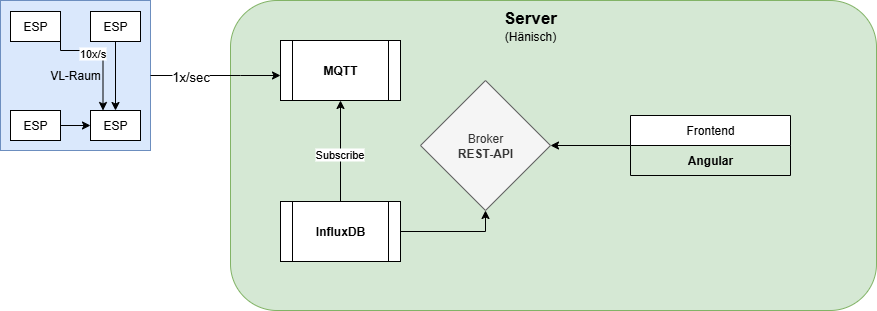
\includegraphics[width=1\textwidth]{../images/MVPVisualisierung.png}
\end{center}

Aufgrundlage des MVPs sollen die folgenden Qualitätsmerkmale sichergestellt werden:
\begin{itemize}
    \item \textbf{Echtheit \& Qualität der Daten:}
    Nur qualitativ "gute" Daten z.B. durch optimierte Mikrofongehäuse ermöglichen realistische Messwerte und damit eine sinnvolle Analyse der akustischen Verhältnisse im Raum.
    \item \textbf{Accountability der Daten:}
    Es muss nachvollziehbar sein, welche Sensoren zu welchem Zeitpunkt welche Daten erfasst haben.
\end{itemize}
